% A LaTeX template for EXECUTIVE SUMMARY of the MSc Thesis submissions to 
% Politecnico di Milano (PoliMi) - School of Industrial and Information Engineering
%
% S. Bonetti, A. Gruttadauria, G. Mescolini, A. Zingaro
% e-mail: template-tesi-ingind@polimi.it
%
% Last Revision: October 2021
%
% Copyright 2021 Politecnico di Milano, Italy. NC-BY

\documentclass[11pt,a4paper,twocolumn]{article}

%------------------------------------------------------------------------------
%	REQUIRED PACKAGES AND  CONFIGURATIONS
%------------------------------------------------------------------------------
% PACKAGES FOR TITLES
\usepackage{titlesec}
\usepackage{color}

% PACKAGES FOR LANGUAGE AND FONT
\usepackage[utf8]{inputenc}
\usepackage[english]{babel}
\usepackage[T1]{fontenc} % Font encoding

% PACKAGES FOR IMAGES
\usepackage{graphicx}
\graphicspath{{Images/}} % Path for images' folder
\usepackage{eso-pic} % For the background picture on the title page
\usepackage{subfig} % Numbered and caption subfigures using \subfloat
\usepackage{caption} % Coloured captions
\usepackage{transparent}

% STANDARD MATH PACKAGES
\usepackage[reqno,fleqn]{amsmath}
\usepackage{amsthm}
\usepackage{bm}
\usepackage[overload]{empheq}  % For braced-style systems of equations

% PACKAGES FOR TABLES
\usepackage{tabularx}
\usepackage{longtable} % tables that can span several pages
\usepackage{colortbl}

% PACKAGES FOR ALGORITHMS (PSEUDO-CODE)
\usepackage{algorithm}
\usepackage{algorithmic}

% PACKAGES FOR REFERENCES & BIBLIOGRAPHY
\usepackage[colorlinks=true,linkcolor=black,anchorcolor=black,citecolor=black,filecolor=black,menucolor=black,runcolor=black,urlcolor=black]{hyperref} % Adds clickable links at references
\usepackage{cleveref}
\usepackage[square, numbers, sort&compress]{natbib} % Square brackets, citing references with numbers, citations sorted by appearance in the text and compressed
\bibliographystyle{plain} % You may use a different style adapted to your field

\usepackage{url}

% PACKAGES FOR THE APPENDIX
\usepackage{appendix}

% PACKAGES FOR ITEMIZE & ENUMERATES 
\usepackage{enumitem}

% OTHER PACKAGES
\usepackage{amsthm,thmtools,xcolor} % Coloured "Theorem"
\usepackage{comment} % Comment part of code
\usepackage{fancyhdr} % Fancy headers and footers
\usepackage{lipsum} % Insert dummy text
\usepackage{tcolorbox} % Create coloured boxes (e.g. the one for the key-words)
\usepackage{stfloats} % Correct position of the tables

%-------------------------------------------------------------------------
%	NEW COMMANDS DEFINED
%-------------------------------------------------------------------------
% EXAMPLES OF NEW COMMANDS -> here you see how to define new commands
\newcommand{\bea}{\begin{eqnarray}} % Shortcut for equation arrays
\newcommand{\eea}{\end{eqnarray}}
\newcommand{\e}[1]{\times 10^{#1}}  % Powers of 10 notation
\newcommand{\mathbbm}[1]{\text{\usefont{U}{bbm}{m}{n}#1}} % From mathbbm.sty
\newcommand{\pdev}[2]{\frac{\partial#1}{\partial#2}}
% NB: you can also override some existing commands with the keyword \renewcommand

%----------------------------------------------------------------------------
%	ADD YOUR PACKAGES (be careful of package interaction)
%----------------------------------------------------------------------------

%----------------------------------------------------------------------------
%	ADD YOUR DEFINITIONS AND COMMANDS (be careful of existing commands)
%----------------------------------------------------------------------------


% Do not change Configuration_files/config.tex file unless you really know what you are doing. 
% This file ends the configuration procedures (e.g. customizing commands, definition of new commands)
% Configuration package
\usepackage[bottom=2.0cm,top=2.0cm,left=2.0cm,right=2.0cm]{geometry}
%\usepackage[bottom=2.0cm,top=2.0cm,left=2.0cm,textwidth=7cm]{geometry}
\raggedbottom 

% Create color bluePoli (-> manuale grafica coordinata:  https://www.polimi.it/fileadmin/user_upload/il_Politecnico/grafica-coordinata/2015_05_11_46xy_manuale_grafica_coordinata.pdf)
\definecolor{bluePoli}{cmyk}{0.4,0.1,0,0.4}

% Custom theorem environments
\declaretheoremstyle[
  headfont=\color{bluePoli}\normalfont\bfseries,
  bodyfont=\color{black}\normalfont\itshape,
]{colored}

\captionsetup[figure]{labelfont={color=bluePoli}} % Set colour of the captions
\captionsetup[table]{labelfont={color=bluePoli}} % Set colour of the captions
\captionsetup[algorithm]{labelfont={color=bluePoli}} % Set colour of the captions

\theoremstyle{colored}
\newtheorem{theorem}{Theorem}[section]
\newtheorem{proposition}{Proposition}[section]

% Enhances the features of the standard "table" and "tabular" environments.
\newcommand\T{\rule{0pt}{2.6ex}}
\newcommand\B{\rule[-1.2ex]{0pt}{0pt}}

% Algorithm description
\newcounter{algsubstate}
\renewcommand{\thealgsubstate}{\alph{algsubstate}}
\newenvironment{algsubstates}{
    \setcounter{algsubstate}{0}%
    \renewcommand{\STATE}{%
    \stepcounter{algsubstate}%
    \Statex {\small\thealgsubstate:}\space}
    }{}
    
% Custom theorem environment
\newcolumntype{L}[1]{>{\raggedright\let\newline\\\arraybackslash\hspace{0pt}}m{#1}}
\newcolumntype{C}[1]{>{\centering\let\newline\\\arraybackslash\hspace{0pt}}m{#1}}
\newcolumntype{R}[1]{>{\raggedleft\let\newline\\\arraybackslash\hspace{0pt}}m{#1}}

% Custom itemize environment
\setlist[itemize,1]{label=$\bullet$}
\setlist[itemize,2]{label=$\circ$}
\setlist[itemize,3]{label=$-$}
\setlist{nosep}

% Create command for background pic
\newcommand\BackgroundPic{% Adding background picture
	\put(237,365){
	    \parbox[b][\paperheight]{\paperwidth}{%
	    \vfill
		\centering
		\transparent{0.4}
		
\includegraphics[width=0.44\paperwidth]{raggiera_polimi.eps}%
		\vfill}
		}
}

% Set indentation
\setlength\parindent{0pt}

% Custom title commands
\titleformat{\section}
{\color{bluePoli}\normalfont\Large\bfseries}
{\color{bluePoli}\thesection.}{1em}{}
\titlespacing*{\section}
{0pt}{3.3ex}{3.3ex}

\titleformat{\subsection}
{\color{bluePoli}\normalfont\large\bfseries}
{\color{bluePoli}\thesubsection.}{1em}{}
\titlespacing*{\subsection}
{0pt}{3.3ex}{3.3ex}

% Custom headers and footers
\pagestyle{fancy}
\fancyhf{}
      
\fancyfoot{}
\fancyfoot[C]{\thepage} % page
\renewcommand{\headrulewidth}{0mm} % headrule width
\renewcommand{\footrulewidth}{0mm} % footrule width

\makeatletter
\patchcmd{\headrule}{\hrule}{\color{black}\hrule}{}{} % headrule
\patchcmd{\footrule}{\hrule}{\color{black}\hrule}{}{} % footrule
\makeatother

% Insert here the info that will be displayed into your Title page 
% -> title of your work
\renewcommand{\title}{A Scalable Solver for the Linearized Poisson-Boltzmann Equation on Cartesian Grids with Hierarchical Local Refinement}
% -> author name and surname
\renewcommand{\author}{Martina Politi}
% -> MSc course
\newcommand{\course}{Mathematical Engineering - Ingegneria Matematica}
% -> advisor name and surname
\newcommand{\advisor}{Prof. Carlo de Falco}
% IF AND ONLY IF you need to modify the co-supervisors you also have to modify the file Configuration_files/title_page.tex (ONLY where it is marked)
\newcommand{\firstcoadvisor}{Dr. Walter Rocchia, Dr. Sergio Decherchi} % insert if any otherwise comment
%\newcommand{\secondcoadvisor}{Dr. Sergio Decherchi} % insert if any otherwise comment
% -> academic year
\newcommand{\YEAR}{2020-2021}

%-------------------------------------------------------------------------
%	BEGIN OF YOUR DOCUMENT
%-------------------------------------------------------------------------
\begin{document}

%-----------------------------------------------------------------------------
% TITLE PAGE
%-----------------------------------------------------------------------------
% Do not change Configuration_files/TitlePage.tex (Modify it IF AND ONLY IF you need to add or delete the Co-advisors)
% This file creates the Title Page of the document
% DO NOT REMOVE SPACES BETWEEN LINES!

\AddToShipoutPicture*{\BackgroundPic}

\hspace{-0.6cm}
\includegraphics[width=0.6\textwidth]{logo_polimi_ing_indinf.eps}

\vspace{-1mm}
\Large{\textbf{\color{bluePoli}{\title}}}\\

\vspace{-0.2cm}
\fontsize{0.3cm}{0.5cm}\selectfont \bfseries \textsc{\color{bluePoli} Tesi di Laurea Magistrale in \\ \course}\\

\vspace{-0.2cm}
\large{\textbf{\author, \ID}}

\small \normalfont

\vspace{11pt}

\centerline{\rule{1.0\textwidth}{0.4pt}}

\begin{center}
\begin{minipage}[t]{.24\textwidth}
\begin{minipage}{.90\textwidth}
\noindent
\scriptsize{\textbf{Advisor:}} \\
\advisor \\
\\
\textbf{Co-advisors:} \\ % leave it if any co-advisor otherwise comment
\firstcoadvisor \\ % leave it if any co-advisor otherwise comment
\secondcoadvisor \\ % leave it if you have more that one co-advisor otherwise comment (if you have more than two co-advisors just copy&paste this line writing \thirdcoadvisor, \fourthcoadvisor, ecc. (REMEMBER to modify also the main.txt)
\\ % leave it if any co-advisor otherwise comment
\textbf{Academic year:} \\
\YEAR \\
\\
\end{minipage}
\end{minipage}% This must go next to `\end{minipage}`
\begin{minipage}{.74\textwidth}
\noindent \textbf{\color{bluePoli} Abstract:} {\abstract}
\end{minipage}
\end{center}

\vspace{15pt}

\begin{tcolorbox}[arc=0pt, boxrule=0pt, colback=bluePoli!60, width=\textwidth, colupper=white]
    \textbf{Key-words:} \keywords
\end{tcolorbox}

\vspace{12pt}

%%%%%%%%%%%%%%%%%%%%%%%%%%%%%%
%%     THESIS MAIN TEXT     %%
%%%%%%%%%%%%%%%%%%%%%%%%%%%%%%

%-----------------------------------------------------------------------------
% INTRODUCTION
%-----------------------------------------------------------------------------
\section{Introduction}
\label{sec:introduction}

This thesis deals with numerical methods and High Performance Computing (HPC) 
Techniques for the computation of the electrostatic potential at the surface
of complex molecules (typically proteins) in aqueous solutions.

The mathematical modeling tool we choose to use for this purpose is the 
Poisson Boltzmann Equation (PBE), which, in mathematical terms, 
is a boundary value problem for a semi-linear elliptic operator with 
discontinuous coefficient and point sources.  

The introduction of such model dates back almost exactly one century ago 
to the seminal work of Born~\cite{ref2}, but its relevance for chemical
and biological applications, {\it e.g.} for drug discovery, still holds~\cite{ref1},
furthermore, when applied to large and complex molecules, such as, {\it e.g.} the 
SARS-CoV-2 spike protein~\cite{ref14}, the solution of the PBE is a challenging 
benchmark for state--of--the--art HPC techniques.
Among  many popular open implementations of PBE solvers we note APBS~\cite{ref3} and 
Delphi~\cite{ref6,ref7,ref7a,ref7b}, the former implements both a Finite Element (FE) 
discretization method on adaptive, conforming, simplicial meshes~\cite{ref4,ref5} 
(more accurate, less efficient) and a Finite Differences (FD) scheme on tensor product
cartesian grids, while the latter strongly relies on the benefits of FD difference
schemes on cartesian grids in terms of memory efficiency and scalability.
Here we focus on the performance and scalability  assessment of numerical methods 
for the PBE based on hierarchically refined cartesian 
Oct-tree grids~\cite{ref10,ref11}, which is a topic that received a growing interest
in the research community in recent years~\cite{ref12,ref14,ref15}.

One aspect in the modeling of protein electrostatics by means of the PBE that 
has been shown to play an important role both in terms of accuracy of the results
and of computational efficiency, is that of the geometrical description of molecular
surfaces in this study we consider and compare different approaches for the surface
definition, ranging from those based on implicit level-set representations to those
based on alpha-shapes~\cite{ref8,ref9}.

\section{The Poisson--Boltzmann E\-qua\-tion}
\label{sec:pbe}

%In this section we present the statement of the PBE in semi-linear and linearized form.
%We also show an example of so-called regularized reformulations that allow to remove point sources from the problem.

%\textbf{\textcolor{red}{usare notazione consistente ad es., se (1) e (2) sono in forma adimensionale e (3) in forma dimensionale, non mi torna la relazione tra $\Phi$ e $\varphi$}}

Figure~\ref{fig:1} shows schematically the geometric 
representation
of the solvated molecule that is the basis of the PBE 
modeling approach. In this representation $ \Omega_m $ 
represents the interior of the molecule which is treated as 
a linear dielectric continuum
medium characterized by a relative permittivity 
$\varepsilon_m$,
while the solvent occupies the region $ \Omega_s $ which is
also modeled as a continuum characterized by permittivity 
$\varepsilon_s$ and by a volume density of charge 
$\rho^s(\varphi(x))$
and $\Gamma$ denotes the molecular surface. 
The points $x_i$ denote 
the centers of the atoms composing the molecule, 
where point charges $q_i$
are located.
\begin{figure}[H]
    \centering
    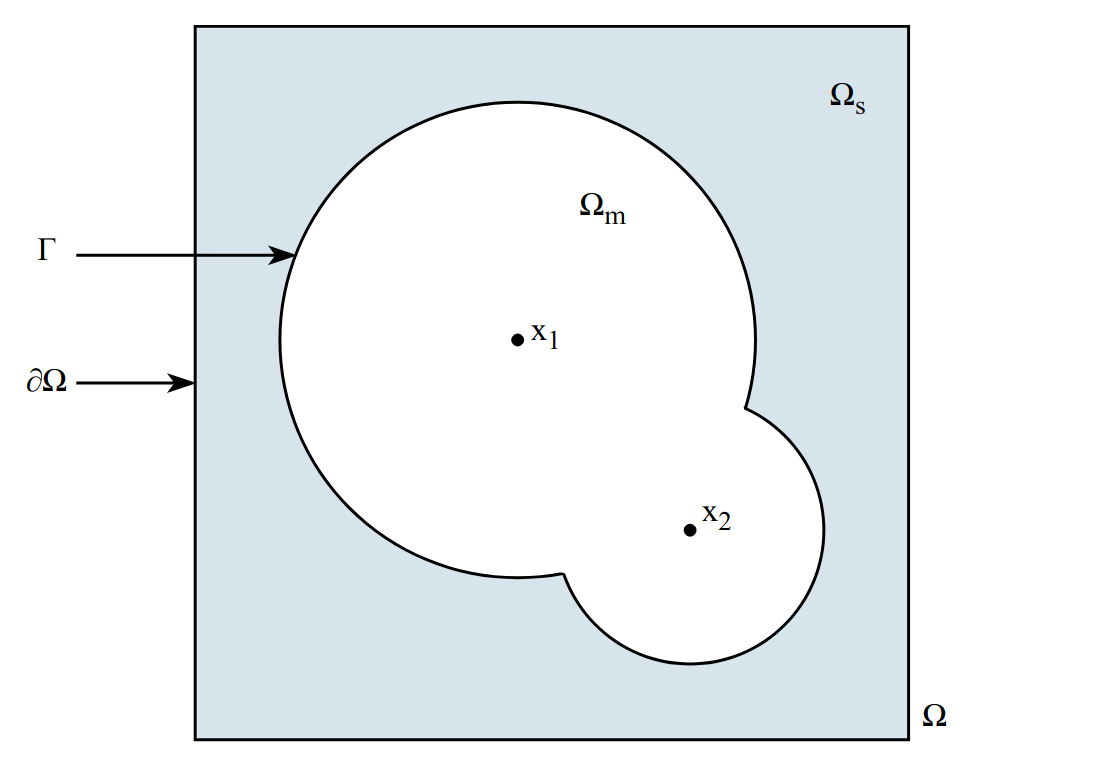
\includegraphics[width=0.47\textwidth]
    {Images/dominio.jpg}
    \caption{Schematic representation of the problem 
    domain.}
\label{fig:1}
\end{figure}
The scalar electrostatic potential $\varphi(x)$ obeys
\begin{equation}
\begin{split}
    \label{eq:pbestart}
    -\nabla \cdot \left(\varepsilon_0\ \varepsilon(x)\ 
    \nabla \varphi(x) \right)  =\
    \rho^s(\varphi(x)) \\ 
    + \sum_i q_i\ \delta(x-x_i),
\end{split}
\end{equation}
which must be complemented by suitable boundary conditions 
on $\partial \Omega$, the most common choice being that of 
homogeneous Dirichlet conditions.

By assuming the charge density in the solvent to obey a 
Maxwell-Boltzmann equilibrium distribution ad by performing
a suitable adimensionalization, \eqref{eq:pbestart}
becomes
\begin{equation}
    \begin{split}
       - &\hat{\nabla} \cdot \left(  
       \hat{\varepsilon}_0\ \varepsilon_r(\hat{x}) \nabla \hat{\varphi}(\hat{x}) 
       \right) + \\ &  \hat{\varepsilon}_0\ \varepsilon_r(\hat{x})\
       \kappa^2(\hat{x}) 
       \sinh\left(\hat{\varphi}(\hat{x})\right)  = 
        \hat{\rho}^f (\hat{x}) ,
        \label{eq:semilinpbe}
    \end{split}
\end{equation}

where the symbol $\hat{\cdot}$ indicates scaled 
nondimensional quantities and will be dropped after this 
section to simplify the notation.



 $\hat{\rho}^f$ in~\eqref{eq:semilinpbe} represents the 
 (scaled) fixed charge density, which is a sum of point 
 sources, while $\hat{\varepsilon}_0 \kappa^2$ is 
 the (scaled) ionic strength.
 


When $\varphi (x)$ is small, one can 
linearize~\eqref{eq:semilinpbe} so that it 
reduces to 
\begin{equation}
    \begin{split}
        -\hat{\nabla} \cdot \left(
        \hat{\varepsilon}_0\ \varepsilon_r\  \hat{\nabla} \hat{\varphi} 
        \right) +  \hat{\varepsilon}_0\ \varepsilon_r\ \kappa^2\ 
        \hat{\varphi}
        = \hat{\rho}^f,
        \label{eq:linpbe}
    \end{split}
\end{equation}
where the dependency on $x$ has been dropped for sake of 
brevity.

Equation~\eqref{eq:linpbe} is known as the \emph{linearized 
PBE} and is the object of the study carried out in the 
present thesis.

At least two different values of $\varepsilon_r$ are needed 
for a decent description of the system physic. 
Indeed, the solvent (in particular water) 
is more sensitive to the presence of an electric field, so 
that the corresponding $\varepsilon_r$ will be higher than 
the solute one. 
The ratio between relative permittivity values in the solute and in the molecule is often of about two orders of 
magnitude, therefore the problem can be considered 
one with \emph{high contrast}.

The most challenging issues to be dealt with in solving~\eqref{eq:linpbe}  are
\begin{enumerate}
    \item the very large size and complex structure of the molecules being studied;
    which lead to very large scale algebraic systems of equations and demand  for state-of-the-art
    HPC solver technology,
    \item the complex geometry of the molecular surface, across which coefficient discontinuities
    occur;
    \item the presence of point sources that lead to singularities in the problem coefficients and solutions.
\end{enumerate}

We will briefly describe the approaches we a\-dop\-ted in order to tackle each of such issues in the following sections.

\section{Treatment of Point Sources}

The simplest approach to deal with the singularities 
introduced by the point sources, is to allow charges 
a \emph{finite volume}, \textit{i.e.} to modify the
fixed charge density by replacing the Dirac $\delta$ 
distributions appearing in~\eqref{eq:pbestart} with
suitable shape functions with finite compact support
\begin{equation}
\label{eq:ui}
    \rho^f(x) = q_i u_i(x),\; \mbox{ where }
  \int  u_i(x)\ \mathrm{dx}^3 = 1 
\end{equation}
so that the total (net) amount of charge is preserved.

When~\eqref{eq:linpbe} is to be solved in a space of
Finite Elements $V_h = \mathrm{Span} \left\{ v_k \right\}$,
usually the $u_i$ are expressed in terms of the $v_k$
so that
\begin{equation}
\label{eq:uivk}
u_i(x) = \sum_k w_{ik} v_k(x).
\end{equation}
In the thesis we discuss a simple 
choice for the weights $ w_{ik}$ 
that preserves total charge, while minimizing dependence
of numerical solutions on mesh rotation an translation.

It is worth noting  that point sources can also 
be eliminated from the problem by using
one of the so-called \emph{regularized reformulations} of the PBE (see, {\it e.g.},~\cite{ref16} for a review
on this topic).

To provide an example of the reformulation technique, consider decomposing $\varphi (x)$ as 
$\varphi (x) = \varphi_s (x) + \varphi_m (x)$, where $\varphi_m (x)$  is the
contribution to the electrostatic potential due only to point sources, while $\varphi_s (x)$ accounts
for the correction due to the surface polarization charge related to the discontinuity in the permittivity. 

By means of the latter decomposition, the linearized PBE becomes

\begin{subequations}
    \begin{align*}[left=\empheqlbrace]
    & - \nabla\cdot ( \varepsilon_s  \nabla \varphi_s) = \\ 
    & = \frac{1}{4 \pi \varepsilon_0 \varepsilon_m} \nabla \varepsilon_s \cdot \sum_i \nabla \Big( \frac{q_i}{|x - x_i|} \Big) + \\ 
    & + \frac{\rho_s}{\varepsilon_0} \Big(\varphi_s  + \frac{1}{4 \pi \varepsilon_0 \varepsilon_m} \sum_i \frac{q_i}{|x - x_i |} \Big) & \mbox{ in } \Omega_s \\
    & - \Delta \varphi_s = 0 & \mbox{ in } \Omega_m  \\
    & [[- \varepsilon \nabla \varphi_s \cdot n]]_{\Gamma} = [[ \varepsilon]]_{\Gamma} \nabla \varphi_m \cdot n & \mbox{ on } \Gamma  \\
    & \varphi_s (x) = \frac{1}{4 \pi \varepsilon_0 \varepsilon_m} \sum_i \frac{q_i}{|x - x_i|} & \mbox{ on } \partial \Omega 
    \end{align*}
\end{subequations}

%\textbf{\textcolor{red}{queste definizioni sono gà per la maggior parte date sopra, qui spiega solo che l'effetto delle cariche puntiformi è trasferito nelle condizioni al contorno e nella condizione di salto}}
The obtained system has no point sources, indeed their effect is now transferred to the third and fourth equations, where the interface condition and the boundary conditions are imposed. At the interface the equality between the jumps $[[ \cdot ]]_\Gamma$ of the given quantities across $\Gamma$ is enforced.
Notice that such jumps can be interpreted as a distribution of surface charges on $\Gamma$.  

The main advantage of this regularization technique is
to avoid the need of using small mesh sizes in $\Omega_m$.

\section{Geometric Representation of the Molecular Surface}
\label{sec:surface}

%In this section we introduce two different methods used for the description of the molecular surface geometry, namely {\it blobby surface} and {\it alpha-shapes}.

The molecular surface is the 2D manifold across which the 
relative permittivity $\varepsilon$ has its discontinuity.

A set of different approaches have been proposed in the
literature to construct the geometry of the surface of a molecule, given the atomic centers and radii.

In this thesis,  we consider and compare three different surface definitions, 
schematically shown in Figure~\ref{fig:2}, \textit{i.e.} : 
\begin{enumerate}
    \item {\it Blobby surface};
    \item {\it Skin surface};
    \item {\it Solvent Excluded Surface} (SES), most commonly known as Connolly surface.
\end{enumerate}

\begin{figure}[H]  
    \centering
    \subfloat[0.5 level-set, Blobby surface \label{fig:blobby}]
    {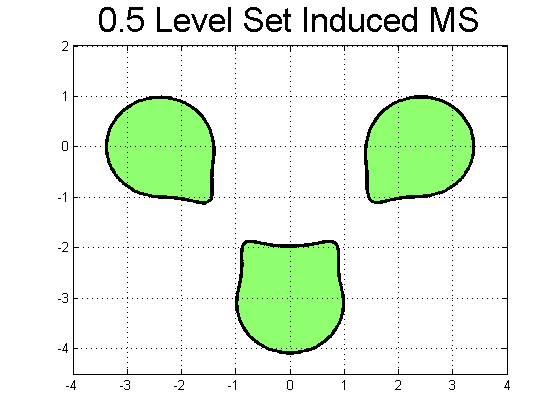
\includegraphics[scale=0.25]{Images/Blobby.jpg}
    }
    \quad
    \subfloat[Skin surface \label{fig:skin}]{
        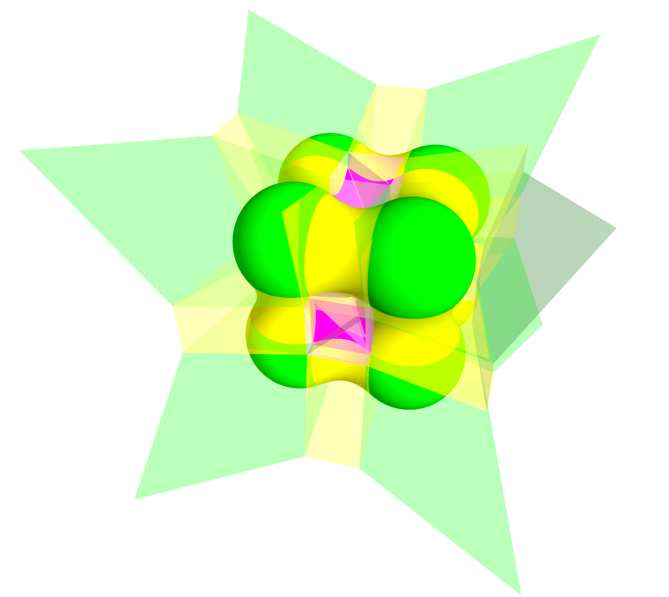
\includegraphics[scale=0.21]{Images/skin.png}
    }
    \quad
    \subfloat[Connolly surface \label{fig:skin}]{
        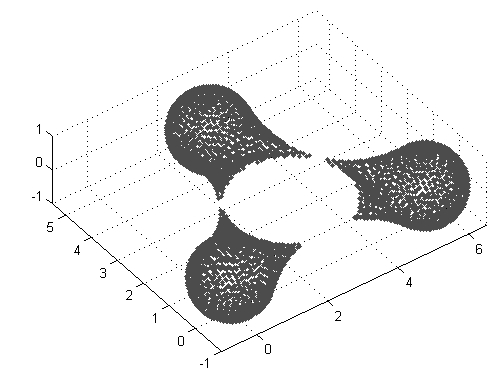
\includegraphics[scale=0.3]{Images/connolly.jpg}
    }
    \caption{Different molecular surfaces \cite{ref8}.} 
    \label{fig:2}
\end{figure}

The first one is based on an implicit level-set representation while the latter two  rely on alpha-shapes.
Alpha-shapes are a parametrized generalization of the convex hull concept.

Figure~\ref{fig:blobbyvsskin} shows the electric potential on a crambin protein simulated using the three different approaches to describe the surface.

%The reasons for the large use of this kind of surface in Computational Biological Chemistry have to be searched in its conceptual simplicity coupled with good results in PBE solution. The limits are the discontinuous dependence of the surface area on the position of atom center and the presence of some singularities in the resulting surface. In order to overcome these problems, the first two molecular surface definitions were proposed. In fact, both {\it Blobby surface} and {\it Skin surface} are appreciated for their smoothness, but while for the first it is difficult to find a good $B$ value, which is crucial for an accurate estimate of the electrostatic potential, the second major drawback is that it can create high dielectric cavities, regions that can affect the energy estimate of the system.  
%For this reasons, up to now, the problem of finding the best molecular surface definition remains a complex problem, for which doesn't exist a unique answer and the choice may vary according to the application context. 

Efficiently constructing the surface and evaluating its interior and exterior region has a significant impact on
the overall simulation complexity, for this reason much
effort during the development of the thesis has been put
in constructing an effective interface with the NanoShaper library~\cite{ref8} to deal with this task.  

\begin{figure*}
    \centering
    \subfloat[Blobby with B = -2.5.]{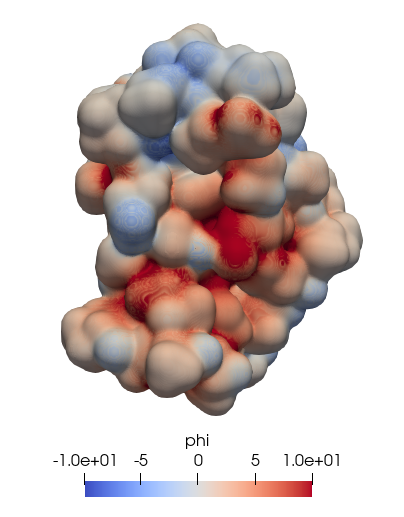
\includegraphics[width=.3\linewidth]{Images/1ccm_blobby_3}}\,
    \subfloat[Skin with s = 0.45.]{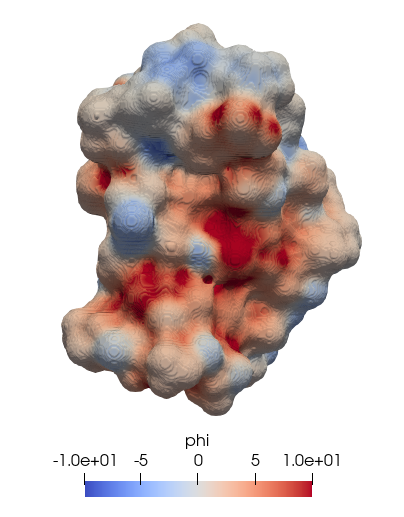
\includegraphics[width=.3\linewidth]{Images/1ccm_skin}}\,
    \subfloat[SES with probe radius 1.4\AA.]{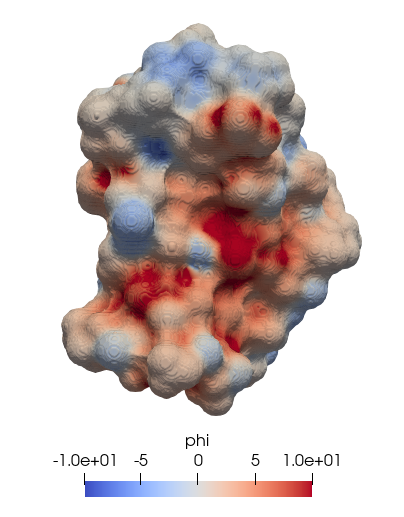
\includegraphics[width=.3\linewidth]{Images/1ccm_ses}}\,
    \caption{Surface for a crambin molecule using different surface representations.}
    \label{fig:blobbyvsskin}
\end{figure*}

\section{Oct-tree grids}
\label{sec:octrees}

%In this sections we introduce the concept of oct-tree grids and their benefits in terms of efficient parallel partitioning, refinement, coarsening and balancing.

The large size and complex structure of the examined molecules leads to
very large scale algebraic systems of equations, which necessitates the usage HPC Techniques. 

Most existing PBE solvers adopt two different kind of grids, either tensor product cartesian grids, or adaptive, simplicial, conforming meshes. Both these options have some advantages and some limitations, in particular the first is characterized by high memory efficiency, but it is not so accurate because it uses simple numerical methods, the second, since the resulting mesh is composed of a very large number of degrees of freedom, is more accurate, but less efficient. The idea for our work was to choose a sort of compromise between the two, solving the linearized PBE with Finite Element method on Oct-tree, which are hierarchically refined, non conforming, cartesian grids. 

In this way we obtained accurate results, given by the adaptive refinement of the mesh, coupled with efficiency, given by the lower number of degrees of freedom in cartesian meshes.   \\
The structure of an Oct-tree grid can be easily represented as a tree, as the name suggests, where each octant ({\it i.e.} each element of the mesh) is a either a leaf or has 8 children, as the Figure \ref{fig:octree} shows. \\
\begin{figure} [H]
    \centering
    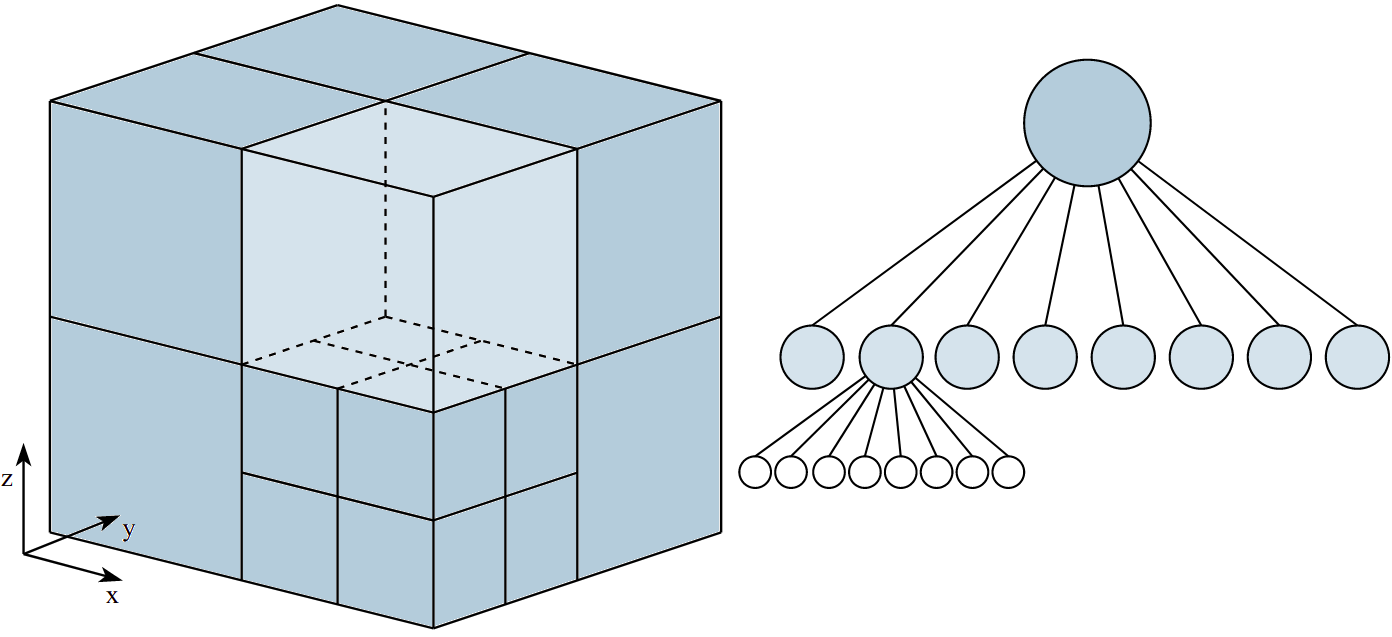
\includegraphics[scale=0.16]{Images/octree_tree}
    \caption{Oct-tree mesh with the corresponding tree.}
    \label{fig:octree}
\end{figure}
A refining-coarsening iterative cycle is performed, starting from a uniform grid, at the end of which the resulting Oct-tree mesh has benefits in terms of efficient parallel partitioning and balancing. 
In particular, parallel partitioning means redistribute the octants present inside the mesh according to a given number of elements per processor or 
according to some prescribed weights associated to those elements. This operation is performed in an efficient way because the resulting element numbering limits communications among processors. For what concerns balancing, it ensures at most 2:1 edge size relations between neighboring octants. This is done in order to properly deal with the {\it hanging nodes}, points belonging to an edge or a face which is refined for two or four elements, but not for the neighboring one. They have to be considered in a different way because don't belong to the set of the degrees of freedom, but are identified through their parents indices. 

\section{Results and Conclusions}
\label{sec:results}

%In this section we show some numerical results obtained with the solver developed during the thesis and some data about the parallel scalability of the code.

%Taking in consideration all the presented aspects, we developed a parallel and scalable PBE solver which integrates the NanoShaper software for dealing with the geometrical surface. 
%In particular we inspected the difference between the results with different molecular surface definition. In Figure \ref{fig:blobbyvsskin}, one can see the resulting electrostatic potential when the chosen surface is produced using the Blobby surface or the Skin one. \\

Even though it has a very long history, 
the use of molecular electrostatics simulations in chemistry
and biology is still an important tool in research today, 
especially as, by making use of cutting-edge HPC techniques,
it allows to simulate ever larger structures.

During this thesis we have developed a parallel solver
for the linearized PBE on adaptive meshes 
and have evaluated its parallel scalability (see Figure~\ref{fig:scaling}) and its viability for 
simulating very large structures of relevance, \textit{e.g.}, for biomedical research (see Figure~\ref{fig:covidVSomicron}).

\begin{figure*}
    \centering
    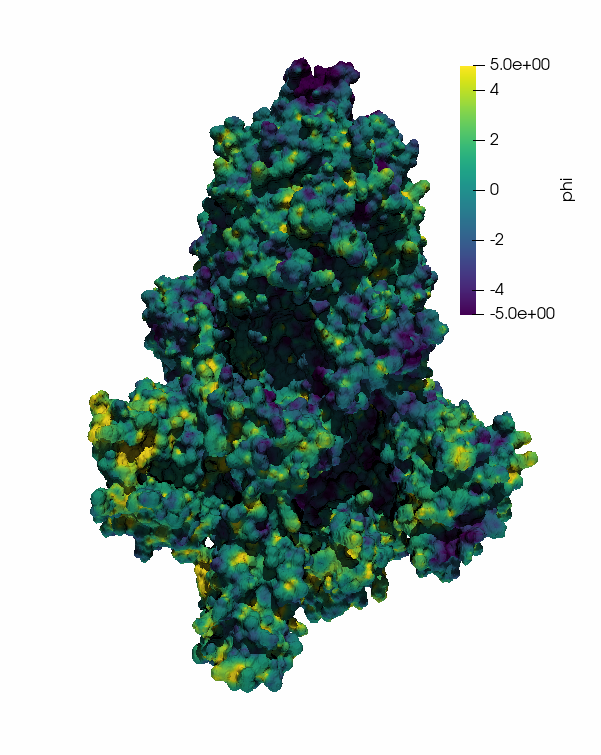
\includegraphics[width=.4\linewidth]{Images/covid} \qquad
    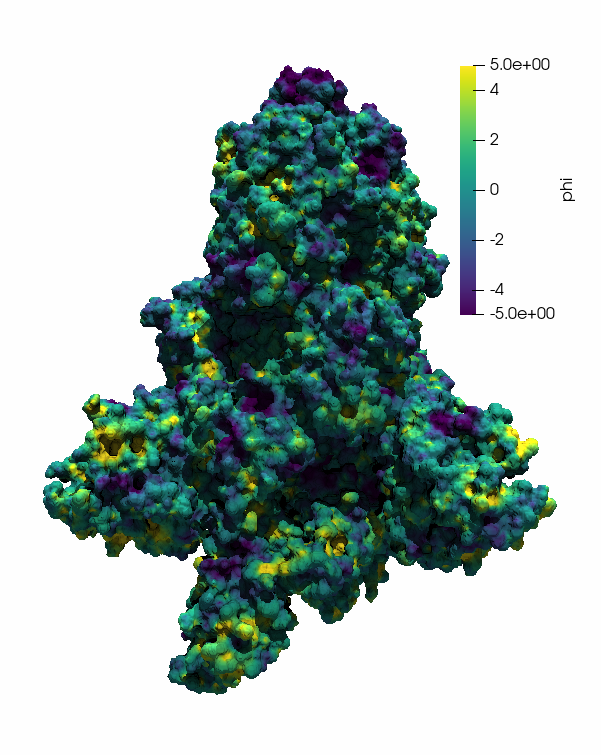
\includegraphics[width=.4\linewidth]{Images/omicron}
    \caption{SARS-CoV-2, spike protein,  ectodomain structure open state (left), 
    Omicron variant of concern (right). One possible application of PBE simulations is that of identifying electrostatic potential patterns that can be useful for automatic drug discovery driven by Artificial Intelligence.}
    \label{fig:covidVSomicron}
\end{figure*}

\begin{figure*}[h]
    \centering
    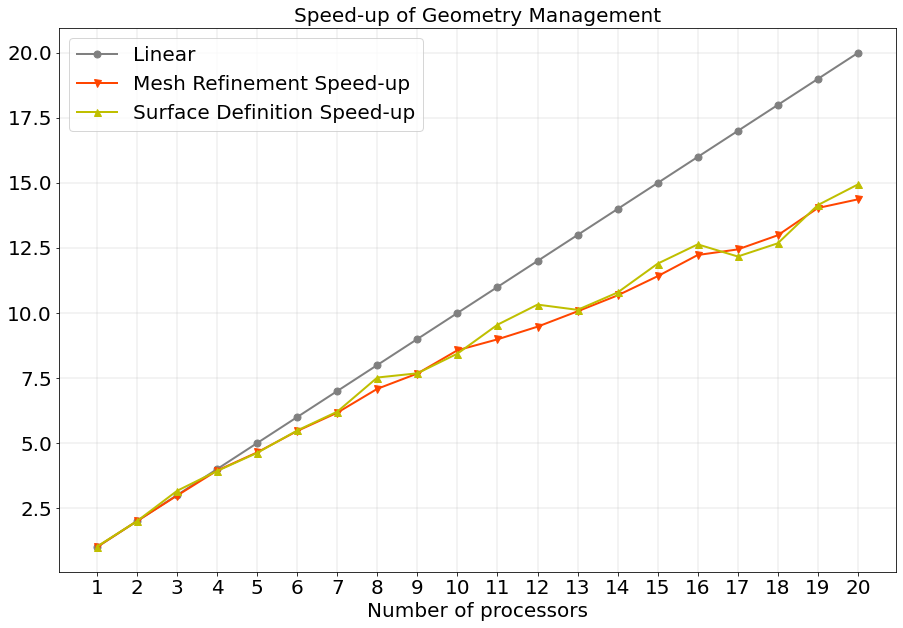
\includegraphics[width=.45\linewidth]{Images/geometry_speedup} \qquad
    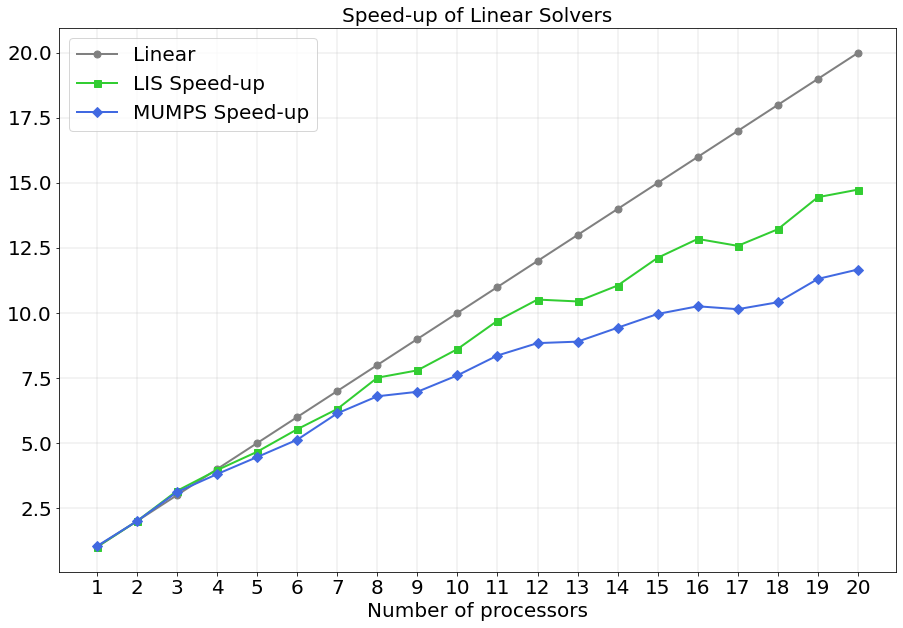
\includegraphics[width=.45\linewidth]{Images/linsolv_speedup}
    \caption{Results of parallel scalability tests that 
    have been performed on the computing server GIGAT of the MOX lab of Politecnico di Milano (6 nodes, 12 Intel Xeon E5-2640v4 @ 2.40GHz, 120 cores, 64GB RAM per node, O.S. CentOS 7
interconnected by a dedicated Gigabit Ethernet).}
    \label{fig:scaling}
\end{figure*}

%---------------------------------------------------------------------------
%  ACKNOWLEDGEMENTS 
%---------------------------------------------------------------------------
\section{Acknowledgements}
We kindly Acknowledge IIT ConceptLAB for interesting discussion and technical support.

%---------------------------------------------------------------------------
%  BIBLIOGRAPHY
%---------------------------------------------------------------------------
% Remember to insert here only the essential bibliography of your work
\nocite{*}
\bibliography{bibliography.bib} % automatically inserted and ordered with this command 

\end{document}